% !TeX spellcheck = de_DE
\section{Verifizierung der Funktionalität}
\label{sec:analysis_valdation_functionality}
Bevor die Analyse aufwendiger Optimierungsprobleme durchgeführt wird, soll die korrekte Funktionalität der sequenziellen Implementierung anhand eines einfachen Beispiels getestet werden. Hierbei liegt der Fokus vor allem auf den strukturellen Mutationen, welche essenziell für größere Probleme sind. Durch eine fehlerhafte Implementierung kann beispielsweise das langfristige Integrieren von neuen erforderlichen Strukturen fehlschlagen. Auch besteht die Möglichkeit, dass ein lokales Maximum durch einen Agenten gefunden wird, dessen Genom dann die restliche Population dominiert, mit der Folge, dass keine neuen Lösungsansätze entwickelt werden können.
\\\\
Um solche Fehler zu entdecken und die korrekte Funktionalität des Algorithmus zu verifizieren, bietet sich das XOR-Problem besonders gut an. Zusätzlich kann ein Vergleich der erhaltenen Ergebnisse mit der originalen Implementierung durchgeführt werden, da auch die Funktionalität von dieser mit dem XOR-Problem verifiziert wurde und die Ergebnisse in Quelle \cite{stanley2002evolving} veröffentlicht sind. Die klassische XOR-Funktion erhält zwei binäre Eingabewerte und erzeugt einen Ausgabewert. Dieser nimmt den Wert $1$ an, wenn genau einer der beiden Eingabewerte $1$ ist. Andernfalls gibt die Funktion den Wert $0$ zurück. Die Abbildung (TODO ABBILDUNG) zeigt links alle möglichen Kombinationen mit zwei Eingabewerten sowie die dazugehörigen Ergebnisse. Rechts in der Abbildung sind die Eingabe- und Ausgabewerte zweidimensional dargestellt. Ziel des XOR-Problems ist, dass ein neuronales Netz für jedes mögliche Paar der Eingabewerte den richtigen Ausgabewert berechnet bzw. den Klassen $0$ und $1$ zuordnet. Durch die Abbildung (TODO ABBILDUNG) ist erkennbar, dass das Unterteilen der Ausgabewerte in die zwei Klassen $0$ und $1$ nicht mit einer linearen Funktion möglich ist. Diese Eigenschaft macht die XOR-Funktion für die Verifizierung der Funktionalität von \ac{NEAT} besonders geeignet. Wie in Kapitel \ref{subsec:network_structures} beschrieben, kann ein \ac{KNN} ohne \emph{Hidden}-Neuronen nur eine lineare Funktion abbilden und ist somit nicht in der Lage, das XOR-Problem zu lösen. Dies trifft auch auf die \ac{KNN} der initialen Population von \ac{NEAT} zu, welche mit einer minimalen Struktur beginnen, die nur aus \emph{Input}- und \emph{Output}-Neuronen besteht. Somit müssen für das erfolgreiche Lösen des XOR-Problems neue Neuronen und Verbindungen erfolgreich in die Population integriert und optimiert werden. 

\subsection{Implementierung}
\begin{figure}
	\begin{python}
		class OptimizationProblemXOR(OptimizationProblem):
		
			xor_tuples = [[0, 0, 0], [1, 0, 1], [0, 1, 1], [1, 1, 0]]
		
			def evaluate(self, neural_network) -> (float, Dict[str, object]):
				fitness_val = 4.0
		
				for xor_input in ChallengeXOR.xor_tuples:
					inputs = [xor_input[0], xor_input[1]]
					result_array = neural_network.activate(inputs)
					result = result_array[0]
					
					fitness_val -= (abs(xor_input[2] - result))
		
		
				# Square remaining fitness
				fitness_val = fitness_val ** 2
				
				return fitness_val, None
	\end{python}
	\label{fig:xor_implementation problem}
	\caption{Implementierung des XOR-Problems in Python}
\end{figure} 
In Abbildung \ref{fig:xor_implementation problem} ist die Implementierung dieses Optimierungsproblems abgebildet, welche im Folgenden genauer erläutert wird. Zu erkennen ist, dass die Implementierung nur wenige Zeilen Programmcode benötigt, was die einfache Nutzung der Bibliothek für verschiedene Optimierungsprobleme verdeutlicht. Zu Beginn des Optimierungsproblems ist eine Liste definiert, welche die verschiedenen Kombinationen der Ein- und Ausgabewerte des XOR-Problems enthält. Danach ist die \emph{evaluate()} Funktion implementiert, welche als Parameter ein initialisiertes \ac{KNN} übergeben bekommt und mit diesem versucht, das XOR-Problem zu lösen. Das \ac{KNN} besitzt entsprechend der später vorgestellten Konfiguration zwei Eingabewerte und einen Ausgabewert. Zum Lösen des Optimierungsproblems wird über die verschiedenen Kombinationen von Eingabewerten iteriert und für jeden Eintrag das \ac{KNN} einmal aktiviert. Das Ergebnis der Aktivierung ist eine Liste, welche in diesem Fall entsprechend der Anzahl an Ausgabeneuronen nur einen Wert enthält und zwar das Ergebnis des \ac{KNN} für die XOR-Funktion. Bei dieser Art der Implementierung wird davon ausgegangen, dass eine Sigmoidfunktion für die Neuronen verwendet wird, sodass das Ergebnis zwischen $0$ und $1$ liegt. Allerdings ist der Ausgabewert allein nicht ausreichend. Wie in den vorherigen Kapiteln beschrieben muss die \emph{evaluate()} Funktion den Fitnesswert berechnen und diesen als Ergebnis zurückgeben. Im nächsten Schritt muss somit die Fitnessfunktion entwickelt werden, welche in diesem Beispiel der Funktion aus Quelle \cite{stanley2002evolving} entspricht. Zu Beginn wird der Fitnesswert entsprechend der Anzahl an Berechnungen auf $4$ initialisiert. Nach jeder Aktivierung wird die Differenz zwischen dem erwarteten und tatsächlich erhaltenen Ergebnis berechnet und anschließend vom Fitnesswert subtrahiert. Da die Differenz aufgrund der Aktivierungsfunktion und der Ausgabewerte zwischen $0$ und $1$ liegen muss, ist der Fitnesswert am Ende der Schleife mindestens $0$ und maximal $4$. Der verbleibende Wert wird danach quadriert, sodass ein besserer Agent einen proportional höheren Fitnesswert erhält \cite{stanley2002evolving}. Am Ende wird dies als Ergebnis der Funktion zurückgegeben. Wie aus der Funktionssignatur zu entnehmen ist, kann optional zusätzlich ein \emph{Dict} übergeben werden, welches Zusatzinformationen enthält. In diesem kann beispielsweise ein \emph{boolean} Wert enthalten sein, welcher anzeigt, ob das \ac{KNN} für alle Eingaben den korrekten Wert berechnet hat. Dieser Wert kann dann beispielsweise für die Abbruchbedingung verwendet werden.


\subsection{Parametrisierung und Ergebnisse}
Die grundsätzliche Implementierung für das XOR-Optimierungsproblem ist im vorherigen Kapitel beschrieben. Bevor das Verfahren durchgeführt wird, sind noch einige grundlegende Parameter zu spezifizieren, welche sich in diesem Beispiel an Quelle \cite{stanley2002evolving} orientieren. Wie bereits beschrieben besitzt jedes \ac{KNN} entsprechend dem Optimierungsproblem zwei Input-Neuronen und ein Output-Neuron. Zusätzlich verwenden alle Neuronen als Aktivierungsfunktion eine modifizierte Sigmoidfunktion, deren Ausgabewert mit $f_{act}(net_j)=\frac{1}{1+e^{-4.9\cdot net_j}}$ berechnet wird. Des Weiteren ist die Abbruchbedingung zu bestimmen. Das Optimierungsverfahren wird beendet, wenn ein \ac{KNN} für alle vier Eingabekombinationen den richtigen Ausgabewert erzeugt. Hierbei wird das Ergebnis als korrekt gewertet, wenn der Ausgabewert $o$ für alle Kombinationen, die $1$ ergeben sollen, $o \geq 0.5$ ist. Dementsprechend muss für alle Kombinationen, die $0$ ergeben sollen, die Bedingung $o < 0.5$ zutreffen. Zusätzlich wird in diesem Durchlauf eine Populationsgröße von $150$ Agenten angenommen. Die Koeffizienten für die in Kapitel \ref{subsec:neat_species} vorgestellte Kompatibilitätsfunktion sind $c_1=1.0$, $c_2=1.0$ und $c_3=0.4$. Ein Genom wird einer Spezies zugeordnet, wenn die berechnete Kompatibilität kleiner als der Schwellwert $\delta_t=3.0$ ist. Auch der in Kapitel \ref{subsubsec:ea_selection} vorgestellte Elitismus wird in dieser Arbeit implementiert. Der beste Agent jeder Spezies, welche mehr als $5$ Mitglieder besitzt, wird unverändert in die nächste Generation kopiert. Des Weiteren erhält eine Spezies nur Nachkommen zugewiesen, wenn in den letzten $15$ Generationen eine Steigerung des maximal erreichten Fitnesswertes erzielt wurde. Zuletzt sind noch die Wahrscheinlichkeiten für die Mutation und Rekombination zu bestimmen. Es besteht für jedes Verbindungsgewicht eine Wahrscheinlichkeit von $80\%$, dass dieses mutiert wird. In diesem Fall wird das Gewicht in $10\%$ der Fälle zufällig neu gewählt, andernfalls wird eine Gauss-Mutation durchgeführt, bei welcher ein Zufallswert auf das Gewicht addiert wird. Zusätzlich besteht für jedes Genom eine Wahrscheinlichkeit von $3\%$, dass ein neues Neuron hinzugefügt wird. Die Wahrscheinlichkeit für eine neue Verbindung liegt bei $5\%$. Bezüglich der Rekombination besteht eine Chance von $25\%$, dass eine Verbindung, welche in beiden Elternteilen deaktiviert ist, im Nachkommen wieder aktiviert wird. 
\\\\ % TODO Evneutll häufiges Wahrscheinlichkeits Wort austauschen
Mit diesen Parametern wird das XOR-Problem $100$ mal nacheinander durchgeführt und die Anzahl an Generationen gemessen, welche zum Lösen des Problems benötigt werden. Die Ergebnisse zeigen, dass im Durchschnitt nach $38$ Generationen ein \ac{KNN} das Optimierungsproblem erfolgreich lösen kann. Im besten Durchlauf wurden $5$ Generationen, im längsten Durchlauf $98$ Generationen benötigt. Aus diesen Ergebnissen ist erkennbar, dass sich die Werte sehr unterscheiden können und dennoch sind in allen $100$ Durchläufen gültige Lösungen gefunden worden. Dass dieses Verhalten nicht ungewöhnlich ist, zeigt ein Vergleich der Ergebnisse mit denen aus der Publikation in Quelle \cite{stanley2002evolving}. Mit der originalen Implementierung werden durchschnittlich $32$ Generationen und im längsten Durchlauf $90$ Generationen zum Lösen des Optimierungsproblems benötigt. Zwar sind die erhaltenen Werte in dieser Arbeit etwas schlechter, die Unterschiede sind jedoch minimal und aufgrund der hohen Varianz der Ergebnisse vernachlässigbar.
\\\\
Das Python Paket mit dem Namen neat-python aus Quelle \cite{mcintyre_neatpython} ist eine weit verbreitete Implementierung des \ac{NEAT} Algorithmus und verwendet eine andere Konfiguration für das XOR-Problem. Zusätzlich sind in dieser Implementierung einige Anpassungen durchgeführt worden, welche eine bessere Performanz bieten sollen. Beispielsweise wird bei der Berechnung des Kompatibilitätswertes standardmäßig die Anzahl an \emph{excess genes} und \emph{disjoint genes} durch den Wert $N$ dividiert. Bei kleinen \ac{KNN} ist dieser Wert $1$ und andernfalls die Größe des \ac{KNN}. Bei der neat-python Implementierung hingegen wird immer durch die Größe des \ac{KNN} dividiert. Zusätzlich ermöglicht diese Implementierung das Nutzen von negativen Fitnesswerten und verwendet bedeutend höhere Wahrscheinlichkeiten für die strukturellen Mutationen. Diese Anpassungen werden für die Implementierung dieser Arbeit übernommen und das XOR-Problem erneut getestet. Die Wahrscheinlichkeit, dass eine neue Verbindung hinzugefügt wird, liegt bei $50\%$ anstelle von $5\%$ bei der originalen Publikation. Ein neues Neuron wird mit einer Wahrscheinlichkeit von $20\%$ hinzugefügt. Zuletzt wird der Faktor $c_3$ der Kompatibilitätsfunktion auf $0.5$ erhöht und die Aktivierungsfunktion geändert. Bei verschiedenen Tests wurden die besten Ergebnisse mit der \ac{tanh} Funktion erzielt. Das Problem wird erneut $100$ mal nacheinander evaluiert und die Anzahl an Generationen zur Lösung gemessen. Mit der vorgestellten Konfiguration werden durchschnittlich $18$ Generationen benötigt bis ein Agent das XOR-Problem erfolgreich löst. Im besten Durchlauf hat ein Agent bereits nach $4$ Generationen eine Lösung gefunden, beim schlechtesten erst nach Generation $49$. Diese Ergebnisse sind im Vergleich zur originalen Implementierung besser. Daher werden die vorgenommenen Änderungen bei den nachfolgenden Verfahren beibehalten.
\begin{figure}[!h]
	\centering
	\begin{minipage}[]{0.49\textwidth}
		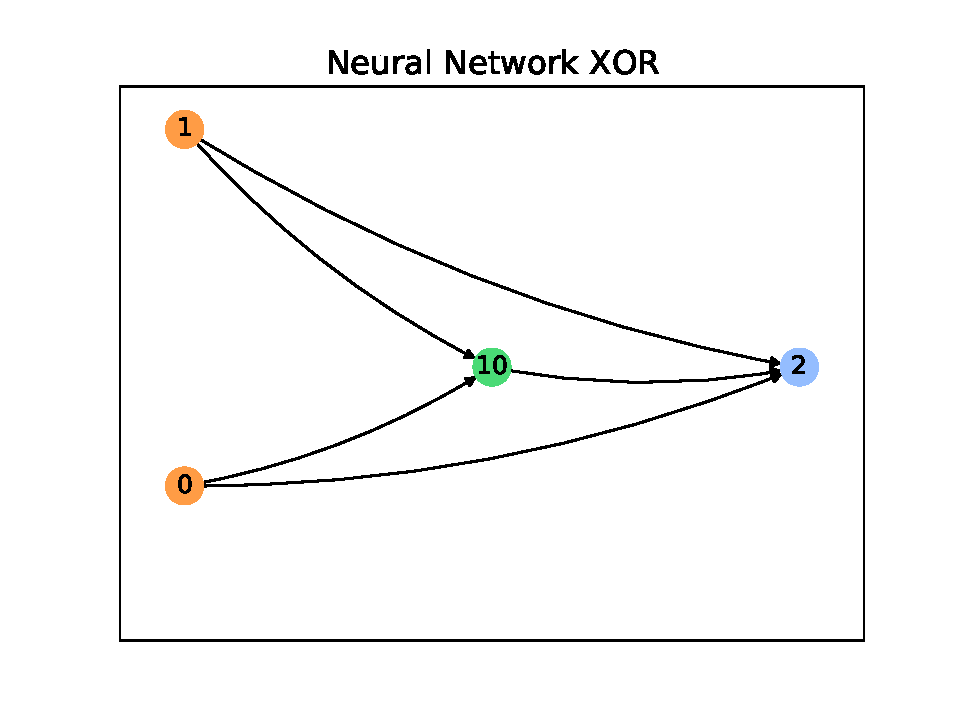
\includegraphics[width=1.0\textwidth]{./img/xor_single_core/xor_neural_network.pdf} 
		%\caption{Lösung für das XOR-Problem mit einem \emph{Hidden}-Neuron}
		%\label{fig:xor_solution_minimal}
	\end{minipage}
	\hfill
	\begin{minipage}[]{0.49\textwidth}
		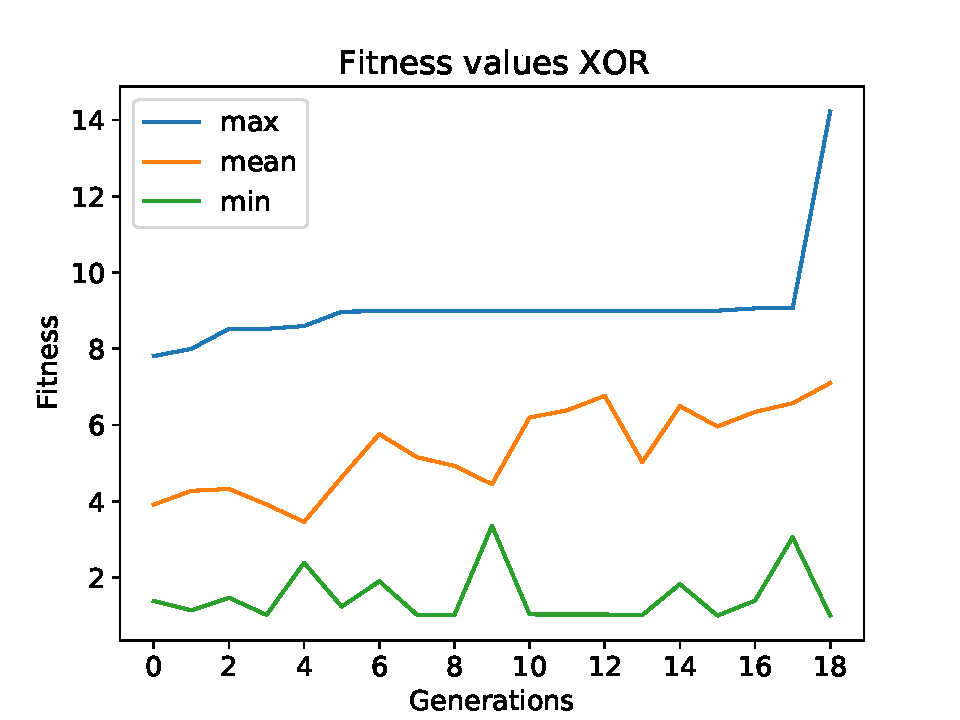
\includegraphics[width=1.0\textwidth]{./img/xor_single_core/xor_fitness.pdf} 
		%\caption{Lösung für das XOR-Problem mit einem \emph{Hidden}-Neuron}
	\end{minipage}
	\caption{Links die Lösung für das XOR-Problem mit einem \emph{Hidden}-Neuron, rechts die dazugehörigen Fitnesswerte pro Generation}
	\label{fig:xor_solution_minimal}
\end{figure}
\\\\
Zuletzt soll die tatsächlich erhaltene Lösung genauer betrachtet werden. Im Durchschnitt hat \ac{NEAT} Lösungen mit 2 oder 3 \emph{Hidden}-Neuronen entwickelt. Allerdings sind auch einige \ac{KNN} entstanden, welche nur ein \emph{Hidden}-Neuron und somit eine minimale Struktur zum Lösen des XOR-Problems besitzen. Ein solch evaluiertes \ac{KNN} ist in Abbildung \ref{fig:xor_solution_minimal} links dargestellt. Die eigentliche Abbildung ist mithilfe der implementierten Visualisierung erstellt worden, welche die Pakete NetworkX und Matplotlib nutzt. Bei solchen Darstellungen ist zu beachten, dass die orangenen Neuronen vom Typ \emph{Input}, die grünen vom Typ \emph{Hidden} und die blauen vom Typ \emph{Output} sind. Die Zahlen auf den Neuronen repräsentieren die jeweilige ID, während die Pfeile die Verbindungen zwischen den Neuronen darstellen. Für eine bessere Übersichtlichkeit wird auf die Darstellung der Gewichte verzichtet. Prinzipiell kann eine solche Abbildung auch gestrichelte Verbindungen enthalten. Diese sind im Genom deaktiviert und werden nicht für die Berechnungen verwendet. In der Abbildung rechts ist der Verlauf des maximalen, minimalen und durchschnittlichen Fitnesswertes für jede Generation dargestellt. Auch diese Abbildung wird mit Matplotlib im Rahmen des implementierten \emph{FitnessReporters} automatisch erstellt und zeigt einige interessante Eigenschaften. Der durchschnittliche Fitnesswert steigt trotz einiger Einbrüche relativ kontinuierlich an. Hieraus lässt sich schließen, dass auch die Population im ganzen Fortschritte erzielt. Der maximale Fitnesswert hingegen stagniert für einige Generationen beim Wert $9$. Der Grund hierfür liegt in der Fitnessfunktion. Ein einfaches \ac{KNN} ohne \emph{Hidden}-Neuronen kann drei Werte des XOR-Problems richtig bestimmen. Ist dies der Fall, ergibt die Fitnessfunktion den Wert $9$. Ab diesem Wert wird kein Fortschritt des Fitnesswertes erzielt bis das neue Neuron erfolgreich in die Struktur integriert ist. Der minimale Fitnesswert ist im gesamten Verlauf sehr gering. Der Grund hierfür ist, dass durch unpassende Mutationen oder Rekombinationen Genome entstehen können, bei denen die negativen Eigenschaften überwiegen. 
\begin{figure}[!h]
	\centering
	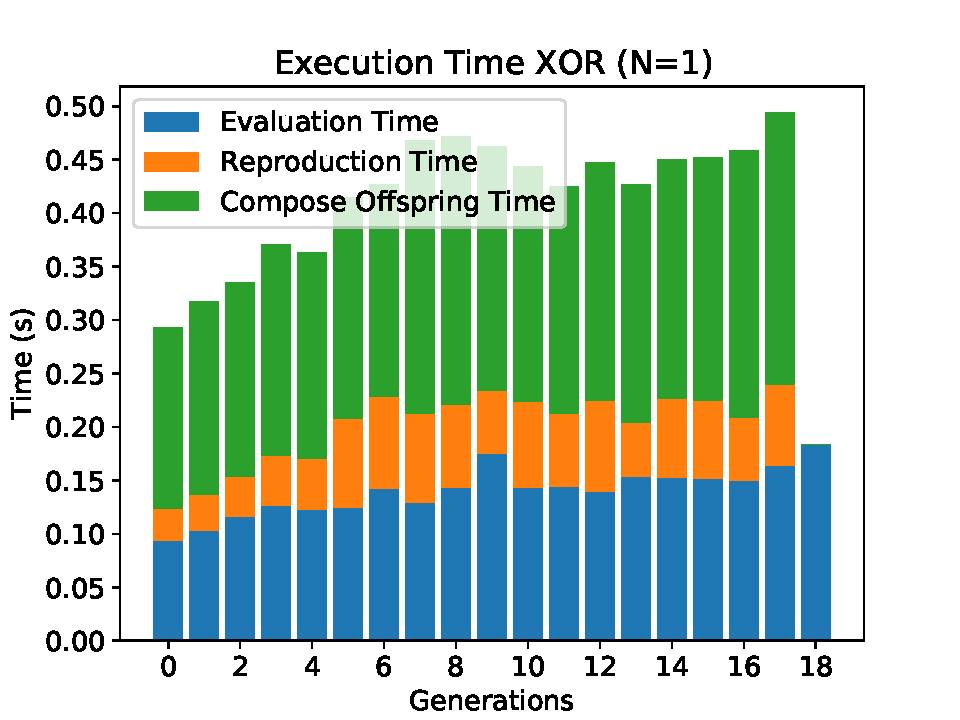
\includegraphics[width=0.5\textwidth]{./img/xor_single_core/xor_execution_time_1.pdf} 
	\caption{Ausführungszeiten des XOR-Problems auf einem Raspberry Pi 4 mit einem Prozess}
	\label{fig:xor_single_core_performance}
\end{figure}
\\\\
Abbildung \ref{fig:xor_single_core_performance} zeigt die Ausführungszeit des Verfahrens in Sekunden für jede Generation. Auch dieser Graph wird wieder automatisch mit dem Paket Matplotlib generiert und zeigt drei verschiedene Phasen. Der blaue Bereich zeigt die \emph{Evaluation Time}, welche die benötigte Evaluationszeit für alle Agenten ist. Der grüne Balken repräsentiert die \emph{Compose Offspring Time}, in welcher die Zeit für die Rekombination und Mutation aller Agenten gemessen wird. Die verbleibenden Aktionen bezüglich \ac{NEAT}, wie zum Beispiel das Sortieren der Agenten in die verschiedenen Spezies, wird im Rahmen der \emph{Reproduction Time} erfasst, welche mit dem orangenen Balken repräsentiert wird. Die benötigte Zeit zum Speichern von Zwischenergebnissen und Erzeugen von Log-Ausgaben wird nicht erfasst, da diese das Ergebnis verfälschen könnten. Insgesamt ist bezüglich des XOR-Problems zu erkennen, dass die Ausführungszeit im Verlauf der Generationen tendenziell ansteigt. Dies kann durch den erhöhten Rechenaufwand erklärt werden, welcher durch größere \ac{KNN} entsteht. Des Weiteren ist auffällig, dass für die letzte Generation keine \emph{Reproduction Time} oder \emph{Compose Offspring Time} erfasst wird. Grund hierfür ist, dass nach der evaluierten Generation die Abbruchbedingung überprüft wird, welche in diesem Fall die Ausführung beendet. Daher wird  keine neue Generation erstellt. Zuletzt soll die allgemeine Ausführungszeit und das Verhältnis der verschiedenen Phasen betrachtet werden. Zu erkennen ist, dass die Ausführungszeit pro Generation weniger als eine halbe Sekunde beträgt. Dies ist vor allem für Testzwecke ein großer Vorteil, da der Effekt von Änderungen schnell zu beobachten ist. Zusätzlich ist zu erkennen, dass die meiste Zeit für das Erstellen und Mutieren von neuen Genomen und Agenten benötigt wird. Allerdings ist diese Verteilung unter Umständen nicht repräsentativ, da die XOR-Funktion ein sehr einfaches Problem ist, welches nur wenige Instruktionen umfasst. Daher werden im nächsten Kapitel aufwendigere Optimierungsprobleme betrachtet.
